% =====================================================================
% Marco Práctico --- Sección 3.8: Fase 3
% =====================================================================

\subsection{Etapa 3 --- Plasticidad Sináptica}
\label{ch:fase3}

Esta fase describe simulaciones de plasticidad LTP/LTD y STDP con modelos
memristivos. Las comparaciones con Jo et al. (2010) se recalcularon con
el protocolo y las particiones descritos abajo, usando puntos
digitalizados de las figuras publicadas. No son mediciones propias ni
certifican por sí solas una respuesta física.

% =====================================================================
\subsubsection{Etapa 3.1: LTP/LTD y STDP}
\label{sec:etapa3_1}

\paragraph{Implementación Cualitativa (LTP/LTD)}
Para estudiar la respuesta acumulativa de la conductancia sináptica (representando el peso lógico $W_{ij}$), se aplicaron secuencias controladas de trenes de pulsos de voltaje idénticos. Matemáticamente, cada pulso induce un minúsculo diferencial $dx$ positivo o negativo sobre el estado del filamento según su polaridad. 

Los pulsos positivos inducen la Potenciación a Largo Plazo (LTP), aumentando la conductancia de forma progresiva. Los pulsos negativos provocan la Depresión a Largo Plazo (LTD), borrando la historia almacenada. La Figura~\ref{fig:20_vi_ltp_ltd} documenta voltaje, corriente, resistencia y conductancia durante pulsos LTP/LTD; la curva temporal escalonada descrita en el informe previo no tiene una figura independiente incluida en este paquete.

El ajuste STDP y sus puntos reservados se muestran en la Figura~\ref{fig:stdp_curve_ch3} del Cap\'itulo~3. Se conserva aqu\'i la interpretaci\'on ampliada de la partici\'on y sus l\'imites.

\textbf{Propósito y Relevancia:} La figura documenta la asimetría del conjunto digitalizado y el error de predicción en los puntos reservados. No certifica la precisión de un cambio de conductancia físico ni la validez general del componente.

\textbf{Curva LTP/LTD atribuida a Jo et al.}
El CSV \texttt{jo2010\_ltp\_ltd.csv} contiene 87 puntos atribuidos por el
validador a la Fig.~2a; no son 200 registros experimentales brutos. Se
simularon 100 pulsos SET de $+3.2\,\mathrm{V}$ y 100 RESET de
$-2.8\,\mathrm{V}$, ambos de $300\,\mu\mathrm{s}$, con lecturas a
$1\,\mathrm{V}$. De los 87 puntos, dos quedan fuera del intervalo de
0--200 pulsos; los 85 restantes se separan, dentro de cada rama, en
bloques contiguos 60/20/20: 50 de entrenamiento, 17 de validación y 18
de test. Se ajustan $R_{\mathrm{on}}$, $R_{\mathrm{off}}$, el coeficiente
de deriva efectivo y $x_0$ solo con entrenamiento; validación selecciona
entre tres inicializaciones. No se aplica un reescalado min--max ni una
calibración afín posterior. En test se obtuvo
$R^2_{\mathrm{residual}}=0.73988$, MAE $=8.3491\,\mathrm{nA}$,
RMSE $=8.6181\,\mathrm{nA}$ y ERP $=31.23\%$. Por rama, el resultado es
deficiente: $R^2=-8.54$ en LTP ($n=10$) y $R^2=-829.99$ en LTD ($n=8$).
Pearson agregado es $r=0.99303$ ($r^2=0.98610$), pero este valor mide
covariación y no sustituye el $R^2_{\mathrm{residual}}$: la predicción
de LTP es constante, por lo que su correlación no está definida; en LTD
se obtiene $r=-0.22170$ ($r^2=0.04915$).
Los parámetros efectivos se ajustan a la misma curva digitalizada y no
son una caracterización independiente del dispositivo; la evidencia es
parcial y no demuestra predicción independiente ni validación completa
del artículo.

La comparaci\'on LTP/LTD y sus puntos reservados se muestran en la Figura~\ref{fig:ltp_ltd_curve_ch3} del Cap\'itulo~3; se conserva aqu\'i el an\'alisis cuantitativo por rama.

\textbf{Propósito y Relevancia:} La figura muestra la forma de la curva bajo la normalización declarada. No demuestra fidelidad física general ni identifica un mecanismo microscópico concreto.


\begin{figure}[H]
    \centering
    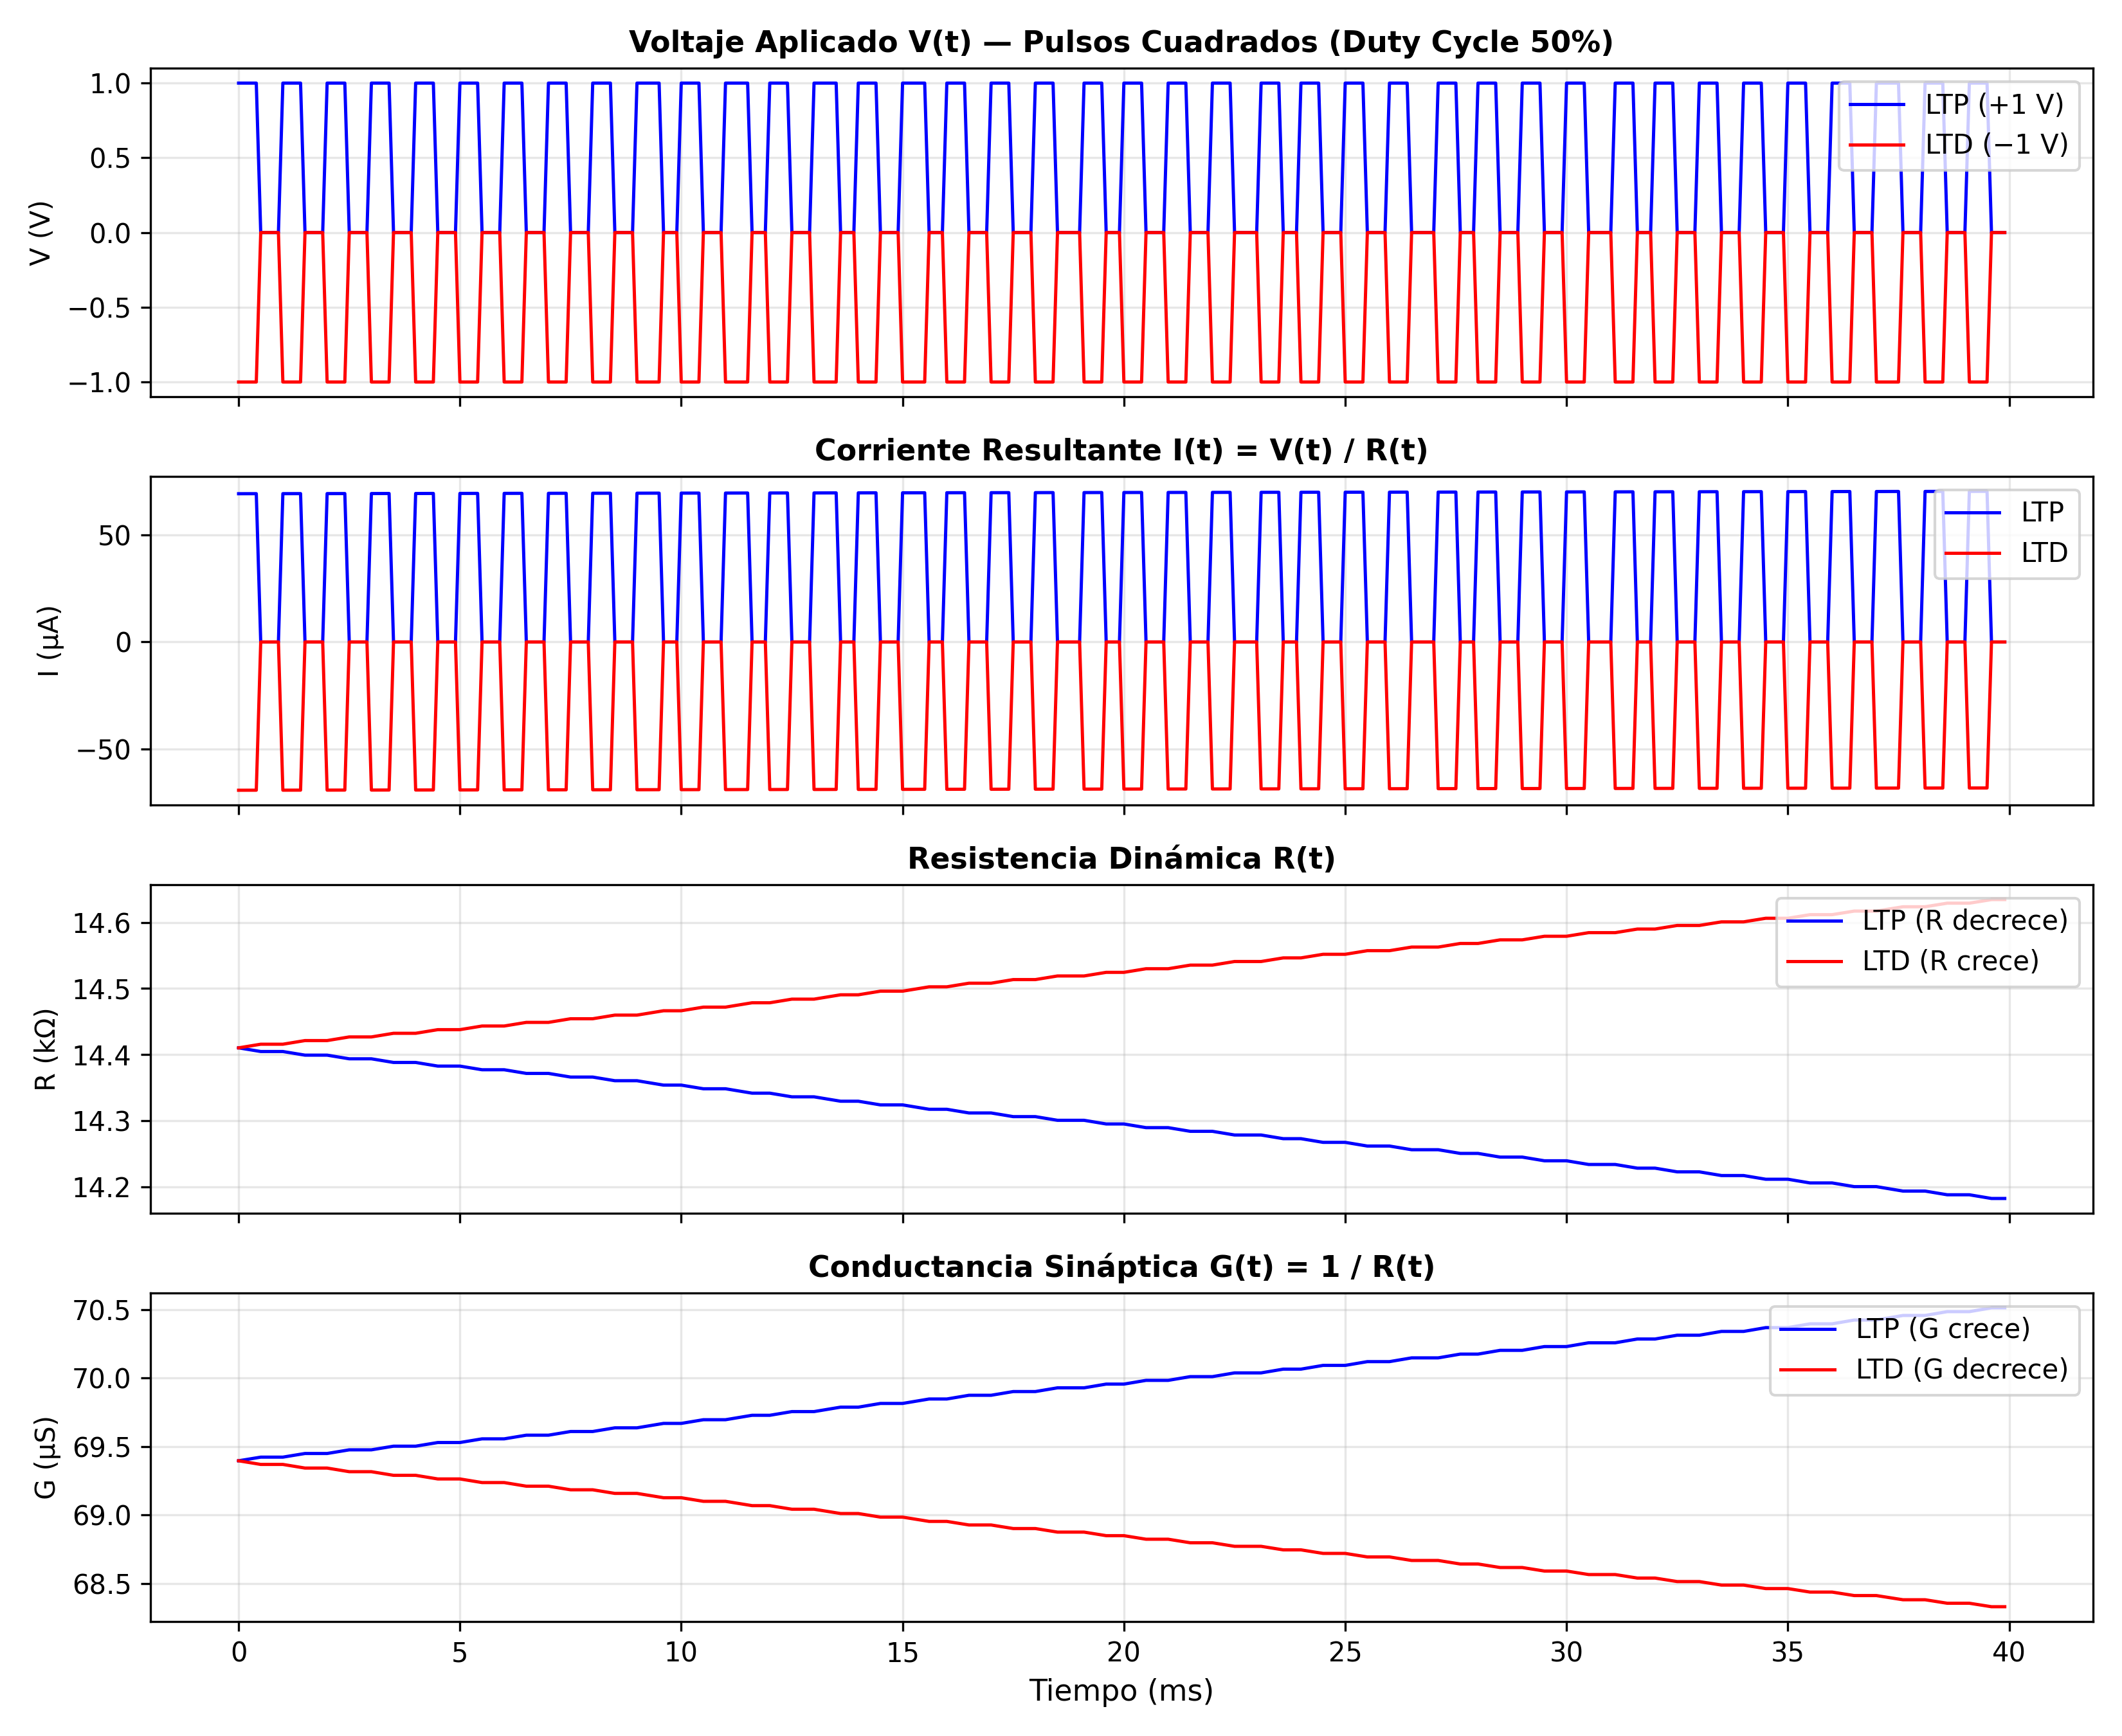
\includegraphics[width=0.7\textwidth]{figuras/fig_20_vi_ltp_ltd.png}
    \caption{Caracterización simultánea de voltaje, corriente, resistencia y conductancia durante pulsos LTP y LTD.}
    \label{fig:20_vi_ltp_ltd}
\end{figure}

\textbf{Propósito y Relevancia:} La figura muestra variables registradas por la simulación durante los pulsos. No constituye una observación microscópica ni una prueba general de conservación para otras configuraciones.
